\documentclass{article}
\usepackage{vaibhavblayer}
\instagramp

\header{160622}{WAV}{01}[E]
\footer{4}

\usetikzlibrary{snakes}
\usepackage{annotate-equations-m}
\begin{document}

\pagecolor{white!85!orange}
\color{white!10!purple}

\title{Doppler's Effect}

\vspace*{\fill}

\begin{center}
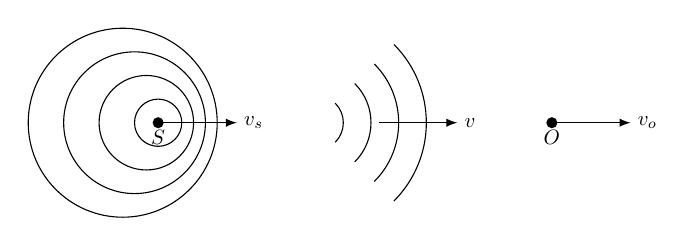
\begin{tikzpicture}[ every node/.style={scale=0.75}]

\coordinate (s) at (0,0);
\coordinate (o) at (5,0);
\coordinate (w) at (2,0);

\fill (s) circle(2pt) node[below]{$S$};
\draw[-latex] (s)--+(1,0) node[right]{$v_s$};
\foreach  \r in {0.3,0.6,...,1.5}
   {
	\draw (s)++(-0.5*\r+0.15, 0) circle[radius=\r];
   };

\fill (o) circle(2pt) node[below]{$O$};
\draw[-latex] (o)--+(1,0) node[right]{$v_o$};
\draw[snake=expanding waves] (w) --+(1.5,0);
\draw[-latex] (w)++(0.8,0)--+(1,0) node[right]{$v$};
\end{tikzpicture}
\end{center}

{\Large
\[
 f' = f_0\left( \dfrac{v \pm v_o}{v \mp v_s} \right)
\]
}
\vspace*{10 mm}

\begin{equation*}
\eqnmarkbox{fn}{f'}
\eqnmarkbox{fo}{f_0}
\eqnmarkbox{v}{v}
\eqnmarkbox{vo}{v_o}
\eqnmarkbox{vs}{v_s}
\end{equation*}
\annotate[yshift=-0.2em]{below, left}{fn}{\texttt{observed frequency}}
\annotate[yshift=-1.2em]{below,left}{fo}{\texttt{source frequency}}
\annotate[yshift=-2.2em]{below,right}{v}{\texttt{velocity of sound in the medium}}
\annotate[yshift=-1.2em]{below,right}{vo}{\texttt{velocity of observer}}
\annotate[yshift=-0.2em]{below,right}{vs}{\texttt{velocity of source}}

\vspace*{\fill}
\end{document}
